\documentclass[
  stu,
  floatsintext,
  longtable,
  a4paper,
  nolmodern,
  notxfonts,
  notimes,
  colorlinks=true,linkcolor=blue,citecolor=blue,urlcolor=blue]{apa7}

\usepackage{amsmath}
\usepackage{amssymb}



\usepackage[bidi=default]{babel}
\babelprovide[main,import]{spanish}
\StartBabelCommands{spanish}{captions} [unicode, fontenc=TU EU1 EU2, charset=utf8] \SetString{\keywordname}{Palabras
Claves}
\EndBabelCommands


% get rid of language-specific shorthands (see #6817):
\let\LanguageShortHands\languageshorthands
\def\languageshorthands#1{}

\RequirePackage{longtable}
\RequirePackage{threeparttablex}

\makeatletter
\renewcommand{\paragraph}{\@startsection{paragraph}{4}{\parindent}%
	{0\baselineskip \@plus 0.2ex \@minus 0.2ex}%
	{-.5em}%
	{\normalfont\normalsize\bfseries\typesectitle}}

\renewcommand{\subparagraph}[1]{\@startsection{subparagraph}{5}{0.5em}%
	{0\baselineskip \@plus 0.2ex \@minus 0.2ex}%
	{-\z@\relax}%
	{\normalfont\normalsize\bfseries\itshape\hspace{\parindent}{#1}\textit{\addperi}}{\relax}}
\makeatother




\usepackage{longtable, booktabs, multirow, multicol, colortbl, hhline, caption, array, float, xpatch}
\setcounter{topnumber}{2}
\setcounter{bottomnumber}{2}
\setcounter{totalnumber}{4}
\renewcommand{\topfraction}{0.85}
\renewcommand{\bottomfraction}{0.85}
\renewcommand{\textfraction}{0.15}
\renewcommand{\floatpagefraction}{0.7}

\usepackage{tcolorbox}
\tcbuselibrary{listings,theorems, breakable, skins}
\usepackage{fontawesome5}

\definecolor{quarto-callout-color}{HTML}{909090}
\definecolor{quarto-callout-note-color}{HTML}{0758E5}
\definecolor{quarto-callout-important-color}{HTML}{CC1914}
\definecolor{quarto-callout-warning-color}{HTML}{EB9113}
\definecolor{quarto-callout-tip-color}{HTML}{00A047}
\definecolor{quarto-callout-caution-color}{HTML}{FC5300}
\definecolor{quarto-callout-color-frame}{HTML}{ACACAC}
\definecolor{quarto-callout-note-color-frame}{HTML}{4582EC}
\definecolor{quarto-callout-important-color-frame}{HTML}{D9534F}
\definecolor{quarto-callout-warning-color-frame}{HTML}{F0AD4E}
\definecolor{quarto-callout-tip-color-frame}{HTML}{02B875}
\definecolor{quarto-callout-caution-color-frame}{HTML}{FD7E14}

%\newlength\Oldarrayrulewidth
%\newlength\Oldtabcolsep


\usepackage{hyperref}




\providecommand{\tightlist}{%
  \setlength{\itemsep}{0pt}\setlength{\parskip}{0pt}}
\usepackage{longtable,booktabs,array}
\usepackage{calc} % for calculating minipage widths
% Correct order of tables after \paragraph or \subparagraph
\usepackage{etoolbox}
\makeatletter
\patchcmd\longtable{\par}{\if@noskipsec\mbox{}\fi\par}{}{}
\makeatother
% Allow footnotes in longtable head/foot
\IfFileExists{footnotehyper.sty}{\usepackage{footnotehyper}}{\usepackage{footnote}}
\makesavenoteenv{longtable}

\usepackage{graphicx}
\makeatletter
\newsavebox\pandoc@box
\newcommand*\pandocbounded[1]{% scales image to fit in text height/width
  \sbox\pandoc@box{#1}%
  \Gscale@div\@tempa{\textheight}{\dimexpr\ht\pandoc@box+\dp\pandoc@box\relax}%
  \Gscale@div\@tempb{\linewidth}{\wd\pandoc@box}%
  \ifdim\@tempb\p@<\@tempa\p@\let\@tempa\@tempb\fi% select the smaller of both
  \ifdim\@tempa\p@<\p@\scalebox{\@tempa}{\usebox\pandoc@box}%
  \else\usebox{\pandoc@box}%
  \fi%
}
% Set default figure placement to htbp
\def\fps@figure{htbp}
\makeatother







\usepackage{newtx}

\defaultfontfeatures{Scale=MatchLowercase}
\defaultfontfeatures[\rmfamily]{Ligatures=TeX,Scale=1}





\title{Exportación de Tuna desde Ayacucho: Un Análisis del Mercado
Internacional}


\shorttitle{EXPORTACIÓN DE TUNA}


\usepackage{etoolbox}


\course{Economía internacional II}
\professor{Econ. William Dante Canales Molina}
\duedate{07/13/2021}

\ccoppy{\textcopyright~2021}





\authorsnames{Edison Achalma,Semnia Chocce,July Durand,Brenda
Gamboa,Alejandrina Galindo}





\affiliation{
{Economía, Universidad Nacional de San Cristóbal de Huamanga}}




\leftheader{Achalma, Chocce, Durand, Gamboa and Galindo}

\date{2021-07-13}


\abstract{This study explores the strategic and ethical considerations
of exporting prickly pear (tuna) from Ayacucho, Peru, to international
markets, with a focus on Beijing, China. It examines the operational
framework of Ecotuna S.C.R.L., a Peruvian company established in 2020,
aiming to penetrate global markets within a year. The analysis includes
market demand in China, logistical processes, and economic viability,
highlighting the fruit's nutritional value and its alignment with
shifting consumer preferences toward healthier diets. Ethical
implications, such as sustainable production and fair trade, are
addressed in the context of contemporary societal needs. Drawing on
trade data and consumer trends, the research underscores the potential
for Ayacucho's tuna to compete with leading exporters like Mexico while
fostering local development. The study concludes by outlining key
challenges and opportunities for sustainable export growth. }

\keywords{prickly pear export, international trade, Ayacucho Peru, China
market, sustainable agriculture}

\authornote{\par{\addORCIDlink{Edison Achalma}{0000-0001-6996-3364}} 
\par{ }
\par{   Los autores no tienen conflictos de intereses que
revelar.    Los roles de autor se clasificaron utilizando la taxonomía
de roles de colaborador (CRediT; https://credit.niso.org/) de la
siguiente manera:  Edison Achalma:   writing, conceptualization; Semnia
Chocce:   formal anlaysis, visualization, editin; July
Durand:   editing, funding acquistion; Brenda Gamboa:   editing, funding
acquistion; Alejandrina Galindo:   editing, funding acquistion}
\par{La correspondencia relativa a este artículo debe dirigirse a Edison
Achalma, Economía, Universidad Nacional de San Cristóbal de
Huamanga, Portla Independencia N
57, Ayacucho, PE, Email: \href{mailto:elmer.achalma.09@unsch.edu.pe}{elmer.achalma.09@unsch.edu.pe}}
}

\makeatletter
\let\endoldlt\endlongtable
\def\endlongtable{
\hline
\endoldlt
}
\makeatother

\urlstyle{same}



\makeatletter
\@ifpackageloaded{caption}{}{\usepackage{caption}}
\AtBeginDocument{%
\ifdefined\contentsname
  \renewcommand*\contentsname{Tabla de contenidos}
\else
  \newcommand\contentsname{Tabla de contenidos}
\fi
\ifdefined\listfigurename
  \renewcommand*\listfigurename{Listado de Figuras}
\else
  \newcommand\listfigurename{Listado de Figuras}
\fi
\ifdefined\listtablename
  \renewcommand*\listtablename{Listado de Tablas}
\else
  \newcommand\listtablename{Listado de Tablas}
\fi
\ifdefined\figurename
  \renewcommand*\figurename{Figura}
\else
  \newcommand\figurename{Figura}
\fi
\ifdefined\tablename
  \renewcommand*\tablename{Tabla}
\else
  \newcommand\tablename{Tabla}
\fi
}
\@ifpackageloaded{float}{}{\usepackage{float}}
\floatstyle{ruled}
\@ifundefined{c@chapter}{\newfloat{codelisting}{h}{lop}}{\newfloat{codelisting}{h}{lop}[chapter]}
\floatname{codelisting}{Listado}
\newcommand*\listoflistings{\listof{codelisting}{Listado de Listados}}
\makeatother
\makeatletter
\makeatother
\makeatletter
\@ifpackageloaded{caption}{}{\usepackage{caption}}
\@ifpackageloaded{subcaption}{}{\usepackage{subcaption}}
\makeatother
\makeatletter
\@ifpackageloaded{fontawesome5}{}{\usepackage{fontawesome5}}
\makeatother

% From https://tex.stackexchange.com/a/645996/211326
%%% apa7 doesn't want to add appendix section titles in the toc
%%% let's make it do it
\makeatletter
\xpatchcmd{\appendix}
  {\par}
  {\addcontentsline{toc}{section}{\@currentlabelname}\par}
  {}{}
\makeatother

%% Disable longtable counter
%% https://tex.stackexchange.com/a/248395/211326

\usepackage{etoolbox}

\makeatletter
\patchcmd{\LT@caption}
  {\bgroup}
  {\bgroup\global\LTpatch@captiontrue}
  {}{}
\patchcmd{\longtable}
  {\par}
  {\par\global\LTpatch@captionfalse}
  {}{}
\apptocmd{\endlongtable}
  {\ifLTpatch@caption\else\addtocounter{table}{-1}\fi}
  {}{}
\newif\ifLTpatch@caption
\makeatother

\begin{document}

\maketitle

\hypertarget{toc}{}
\tableofcontents
\newpage
\section[Introduction]{Exportación de Tuna desde Ayacucho}

\setcounter{secnumdepth}{-\maxdimen} % remove section numbering

\setlength\LTleft{0pt}


\section{Capítulo 1. Antecedentes de la
empresa}\label{capuxedtulo-1.-antecedentes-de-la-empresa}

\subsection{Historia de la empresa}\label{historia-de-la-empresa}

LA EMPRESA ECOTUNA S.C.R.L. es una empresa peruana dedicada a la
exportación de tuna, de la más alta calidad, saludable y buen sabor. Fue
creada y fundada el 23 de enero del 2020, registrada dentro de las
sociedades mercantiles y comerciales como una sociedad comercial de
responsabilidad limitada.

Con miras a su expansión internacional, Ecotuna proyecta realizar sus
primeras exportaciones en un plazo máximo de un año. Así, la empresa
busca desarrollarse y crecer, tanto en el mercado nacional como
internacional y generar valor a través de la innovación en el
desarrollo. Mejorar los productos que ofrece, con una rápida capacidad
de respuesta, flexibilidad a los requerimientos y necesidades de los
clientes, para la mejora continua de los procesos.

Nuestro equipo está comprometido con la calidad del producto, proceso de
mejora continua y en la construcción de lazos comerciales a largo plazo
con nuestros clientes y stakeholders.

\subsection{Descripción de producto}\label{descripciuxf3n-de-producto}

La tuna, cuyo nombre científico es Opuntia ficus-indica, es una planta
de la familia de las cactáceas la cual crece en los valles secos
interandinos de Ayacucho.

Especialmente adaptada a la escasez de agua y cuya exportación no
compite con las tierras agrícolas. Esta planta produce frutos
comestibles que, con el tiempo, ha llegado a tener gran aceptación en el
mercado. La partida arancelaria es 0810909000.

\begin{figure}

\caption{\label{fig-figura1}}

\centering{

\pandocbounded{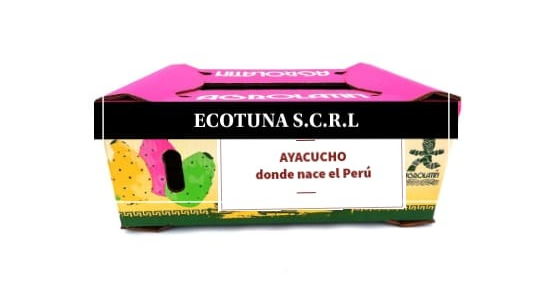
\includegraphics[keepaspectratio]{index_files/figure-html/figura1.png}}

}

\end{figure}%

\textbf{NOMBRE:} Tuna, nopal, chumbera, penca

\textbf{DESCRIPCIÓN}: Tuna

\textbf{PRESENTACIÓN:} Principalmente como fresco, también puede
industrializarse con la perspectiva de procesar agroindustrialmente a la
elaboración de jugos y pulpas, fruta deshidratada, aceites y gomas,
mermeladas y néctares.

\textbf{ESPECIES Y VARIEDADES:} En nuestro país, se conocen las
siguientes variedades: tuna rosada.

\textbf{ZONAS DE PRODUCCIÓN:} La tuna en nuestro país es producida
principalmente en los departamentos de \textbf{Ayacucho}, Huancavelica,
Lima y Cusco

\textbf{ORIGEN:} La tuna es originaria de los Andes del Perú, Bolivia y
de las planicies de México.

\textbf{USOS Y APLICACIONES:} Proviene de una planta con 1.5 - 2.5 m. de
altura, flores color amarillo claro, pencas de 20 - 25 cm de diámetro.
Es una planta susceptible a plagas y enfermedades

\section{Capítulo 2. Plan estratégico y plan
organizacional}\label{capuxedtulo-2.-plan-estratuxe9gico-y-plan-organizacional}

\subsection{Gestión administrativa}\label{gestiuxf3n-administrativa}

El objetivo de la administración es aumentar la productividad como medio
para incrementar las posibilidades de competir con éxito en el mercado
de Estados Unidos. La gerencia se encargará de manejar los aspectos no
solo operacionales, sino también estratégicos, así como de definir el
rumbo y las estrategias de la organización.

En el Organigrama de la empresa ECOTUNA, se deben destacar las
siguientes instancias:

\begin{itemize}
\item
  Asamblea General de delegados.
\item
  Consejo Directivo.
\item
  Gerencia.
\item
  Comités Consultivos.
\end{itemize}

\subsection{Gestión de los mercados internacionales y logística
exportadora}\label{gestiuxf3n-de-los-mercados-internacionales-y-loguxedstica-exportadora}

\subsubsection{Proceso Logístico País
Exportador}\label{proceso-loguxedstico-pauxeds-exportador}

Se desarrollará la compra de tunas al por mayor de regiones estratégicas
que producen la tuna con lo cual tendremos la capacidad necesaria para
abastecer el mercado internacional.

\textbf{Protocolo del producto}. Después se realiza la cadena de
embalaje del producto Tuna, el cual va a hacer embalado en cajas para
frutas con ranura de ventilación y circulación a frío.

\textbf{Protocolo de Embalaje.} El embalado de tuna será en cajas para
frutas, que llevara una ranura de ventilación y circulación a frio.

\begin{figure}[H]

\caption{Protocolo de Embalaje}

{\centering \pandocbounded{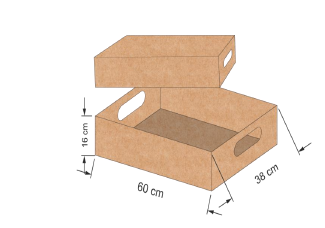
\includegraphics[keepaspectratio]{index_files/figure-html/figura2.png}}

}

\end{figure}%

\textbf{Protocolo de Embarque}. La mercancía será cargada en el almacén
de nuestra empresa ECOTUNA en el departamento de Ayacucho, que luego
será llevado en camiones con destino al aeropuerto internacional del
Perú donde será la carga de la mercancía de 1500 cajas a un contenedor.

\begin{figure}[H]

\caption{Protocolo de Embarque}

{\centering \pandocbounded{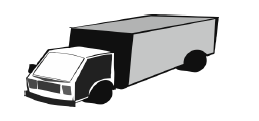
\includegraphics[keepaspectratio]{index_files/figure-html/figura3.png}}

}

\end{figure}%%
\begin{figure}[H]

\caption{Alt text}

{\centering \pandocbounded{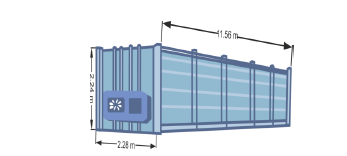
\includegraphics[keepaspectratio]{index_files/figure-html/figura4.png}}

}

\end{figure}%

\subsubsection{Logística del Trayecto de
Origen}\label{loguxedstica-del-trayecto-de-origen}

Para la exportación de Tuna, el vendedor debe entregarle al agente de
adunas la siguiente información previamente diligenciada:

· Factura de venta

· Lista de empaque

· Certificado de origen

· Mandato aduanero

\paragraph{Trayecto internacional.}\label{trayecto-internacional}

\begin{enumerate}
\def\labelenumi{\arabic{enumi}.}
\item
  Obtención de la fecha del zarpe del avion desde el aeropuerto
  internacional y certificación de la fecha del ETA (Stimetion time
  arrive) del avion a Beijin.
\item
  Reclamación de los documentos originales en la línea aérea.
\item
  Contratación de flete aéreo internacional.
\item
  La contratación de seguro internacional será pagada por el importador
  de acuerdo con nuestro INCOTERM.
\end{enumerate}

\paragraph{Trayecto destino.}\label{trayecto-destino}

El destino es Beijín

\begin{figure}[H]

\caption{Trayecto destino}

{\centering \pandocbounded{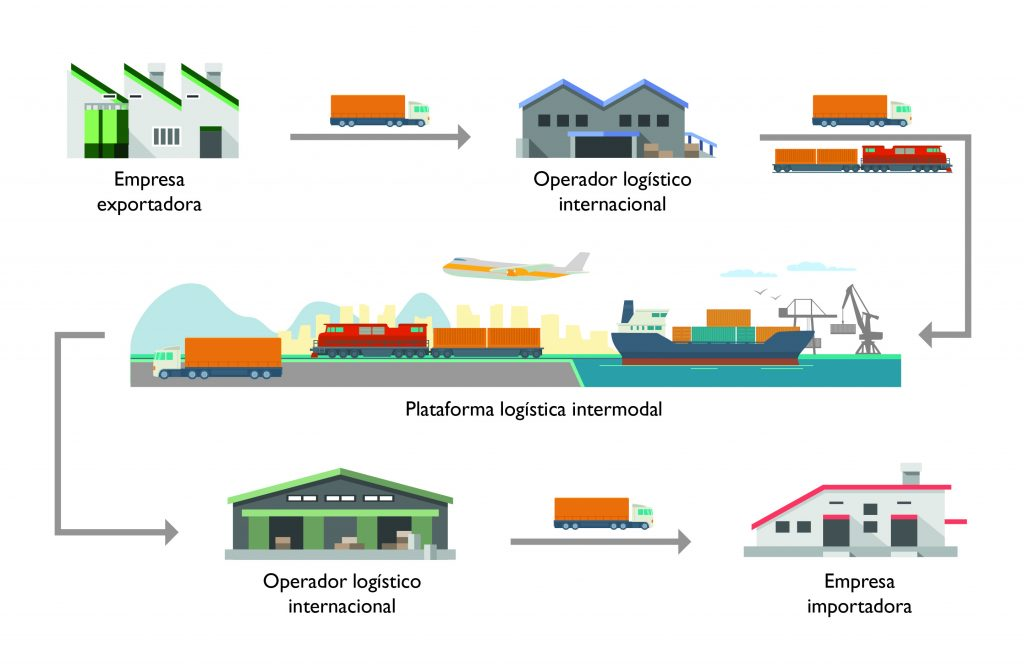
\includegraphics[keepaspectratio]{index_files/figure-html/figura5.jpg}}

}

\end{figure}%

\subsubsection{Gestión económica y
financiera}\label{gestiuxf3n-econuxf3mica-y-financiera}

Como base para cualquier negocio, es necesario disponer de una fuente de
capital que ayude en el inicio y posterior comienzo de la actividad. Se
podrá exportar con la ayuda de las siguientes fuentes:

\begin{itemize}
\item
  Fuentes ajenas: Préstamos financieros, del banco Interbank.
\item
  Fuentes propias: Aportación de los socios.
\item
  Ayudas públicas: Financiación por parte de los organismos públicos.
\end{itemize}

\subsection{Plan estratégico}\label{plan-estratuxe9gico}

\subsubsection{Misión}\label{misiuxf3n}

Exportación de Tuna a los mercados internacionales como China y la
comunidad europea, superando las expectativas de nuestros clientes
internacionales, en cuanto a sabor, frescura e inocuidad alimentaria.

\subsubsection{Visión}\label{visiuxf3n}

Para el año 2023, ser reconocidos internacionalmente, como una empresa
exportadora de tuna de la mejor calidad; ampliando la cartera de
productos rentables y diversificados, propietarios de terrenos
debidamente manejados e ingresando a los mercados más exigentes del
mundo, caracterizándonos por la alta calidad y frescura de nuestros
productos, generando valor y bienestar a nuestros colaboradores, a
nuestros proveedores y a nuestros clientes.

\subsection{Plan de marketing}\label{plan-de-marketing}

\section{Capítulo 3. Estudio de mercado internacional y plan de
marketing}\label{capuxedtulo-3.-estudio-de-mercado-internacional-y-plan-de-marketing}

\subsection{Análisis de la oferta}\label{anuxe1lisis-de-la-oferta}

\begin{table}

{\caption{{Principales países exportadores}{\label{tbl-mytableppe}}}}

\begin{longtable}[]{@{}
  >{\raggedright\arraybackslash}p{(\linewidth - 8\tabcolsep) * \real{0.2000}}
  >{\raggedright\arraybackslash}p{(\linewidth - 8\tabcolsep) * \real{0.2000}}
  >{\centering\arraybackslash}p{(\linewidth - 8\tabcolsep) * \real{0.2000}}
  >{\centering\arraybackslash}p{(\linewidth - 8\tabcolsep) * \real{0.2000}}
  >{\centering\arraybackslash}p{(\linewidth - 8\tabcolsep) * \real{0.2000}}@{}}
\toprule\noalign{}
\begin{minipage}[b]{\linewidth}\raggedright
\textbf{Nº}
\end{minipage} & \begin{minipage}[b]{\linewidth}\raggedright
\textbf{País}
\end{minipage} & \begin{minipage}[b]{\linewidth}\centering
\textbf{\%Var 18-17}
\end{minipage} & \begin{minipage}[b]{\linewidth}\centering
\textbf{\%Part 18}
\end{minipage} & \begin{minipage}[b]{\linewidth}\centering
\textbf{Total Exp. 2018 (millon US\$)}
\end{minipage} \\
\midrule\noalign{}
\endhead
\bottomrule\noalign{}
\endlastfoot
1 & Mexico & 106\% & 79\% & 200.22 \\
2 & Italia & 29\% & 12\% & 272.47 \\
\end{longtable}

{\noindent \emph{Note.} COMTRADE}

\end{table}

\begin{figure}[!htbp]

{\caption{{Participación en la produción de
tuna}{\label{fig-myimportedimage}}}}

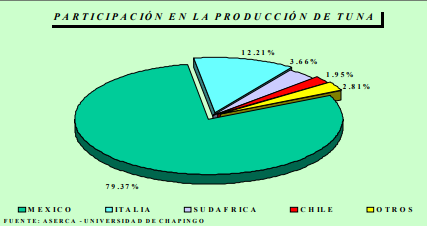
\includegraphics[width=5in,height=\textheight,keepaspectratio]{index_files/figure-html/figura6.png}

{\noindent \emph{Note.} ASERCA - Universidad de Chapingo}

\end{figure}

México al ser el país de origen de este fruto cuenta con la ventaja de
tener un depositario nacional con más de 400 variedades de tuna. De un
total de 40.000 toneladas de~\textbf{tuna}~que se exportan
aproximadamente, Puebla aporta 8.000. Por tanto, se considera como una
competencia para nuestra empresa.

\begin{table}

{\caption{{Principales empresas exportadoras}{\label{tbl-mytablepee}}}}

\begin{longtable}[]{@{}
  >{\raggedright\arraybackslash}p{(\linewidth - 4\tabcolsep) * \real{0.5507}}
  >{\centering\arraybackslash}p{(\linewidth - 4\tabcolsep) * \real{0.2319}}
  >{\centering\arraybackslash}p{(\linewidth - 4\tabcolsep) * \real{0.2174}}@{}}
\toprule\noalign{}
\begin{minipage}[b]{\linewidth}\raggedright
\textbf{Empresa}
\end{minipage} & \begin{minipage}[b]{\linewidth}\centering
\textbf{\%Var 20-19}
\end{minipage} & \begin{minipage}[b]{\linewidth}\centering
\textbf{\%Part. 20}
\end{minipage} \\
\midrule\noalign{}
\endhead
\bottomrule\noalign{}
\endlastfoot
Empresa Mexbest Mexico & 20\% & 17\% \\
Empresa TunaMex & & \\
Pomica Perú sociedad anónima cerrada & 7\% & 7 \\
\end{longtable}

\end{table}

\subsection{Mercado objetivo}\label{mercado-objetivo}

Nuestro mercado de destino será China específicamente su capital Beijín,
este país es uno de los principales importadores de tuna (partida frutas
frescas), pues importa el 41\% de tuna a nivel mundial, dicha ciudad
cuenta con un estimado de 18,827,069 de habitantes al 2020 de acuerdo
con los datos de la CEPAL con un aumento de 0, 47\% promedio anual.

\subsection{Ficha país}\label{ficha-pauxeds}

\begin{longtable}[]{@{}
  >{\raggedright\arraybackslash}p{(\linewidth - 2\tabcolsep) * \real{0.4225}}
  >{\raggedright\arraybackslash}p{(\linewidth - 2\tabcolsep) * \real{0.5775}}@{}}
\toprule\noalign{}
\begin{minipage}[b]{\linewidth}\raggedright
\textbf{País objetivo}
\end{minipage} & \begin{minipage}[b]{\linewidth}\raggedright
\textbf{CHINA}
\end{minipage} \\
\midrule\noalign{}
\endhead
\bottomrule\noalign{}
\endlastfoot
\textbf{Área} & 9.562.910 Km2 \\
Capital & Beijing - Pekín \\
Población & 1.400.050.000 \\
\textbf{Idioma oficial} & Mandarín \\
Ubicación geográfica & Asia \\
Moneda & Yuanes chinos \\
\textbf{Tipo de cambio} & 0.15 USD -0.61 PEN \\
Pbi & 12.901.904 M.€ - 15255791.88 Mill USD \\
\textbf{Pbi per cápita} & 9.215€ - 10.89 USD \\
Tasa de crecimiento anual & 18,3\% \\
Clima & En China, los veranos son largos, tórridos, opresivos y
ventosos; los inviernos son cortos, frescos y secos y está parcialmente
nublado durante todo el año. Durante el transcurso del año, la
temperatura generalmente varía de 10 °C a 37 °C y rara vez baja a menos
de 4 °C o sube a más de 39 °C. \\
\textbf{Pesos y medidas} & Jin \\
\textbf{Días festivos} & 01 de enero, El día de año nuevo \\
& 12- 17 de febrero, Año nuevo chino \\
& 3 -- 5 de abril, Festival Qing Ming \\
& 14 al 16 de junio, Festival del barco del dragón \\
& El 21 de setiembre, Festival de mediados de otoño \\
& De 1- 7 de octubre, Dia nacional de la semana dorada \\
\end{longtable}

\subsection{Exigencias del producto}\label{exigencias-del-producto}

\subsubsection{Requisitos de
importación}\label{requisitos-de-importaciuxf3n}

Para las exportaciones realizadas desde/a China se deben presentar los
siguientes documentos:

\begin{itemize}
\item
  declaración de aduanas, contrato original (con sello), factura
  comercial original (con sello), lista de empaque original (con sello),
  certificado de salida y certificación de cuarentena, documentos de
  transporte, documentos de seguro, Documentos legales
\item
  Código de Registro de Aduanas (Código CR): Para todos los envíos
  (excepto documento y efectos personales) deben estar identificados con
  dicho código.
\item
  Código Armonizado (Código HS): El código HS ayuda a clasificar las
  mercancías y acelerar el despacho de aduanas.
\end{itemize}

Todas las empresas de los países autorizados para exportar a China deben
registrarse ante AQSIQ. Los documentos de recomendación incluyen:

\begin{itemize}
\item
  Información de la compañía. Nombre/dirección/ n° aprobación
\item
  Información del producto: Nombre/materias primas/aplicación
\item
  Certificado de libre venta emitido por el organismo nacional del país
  de origen
\end{itemize}

Los productos que arriben a China podrán ser destruidos o devueltos si
se encuentra cualquiera de las siguientes condiciones:

\begin{itemize}
\item
  El país de origen se encuentra prohibido de exportar a China
\item
  Los proveedores (exportadores) no cuentan con aún con la licencia
  china
\item
  El producto del proveedor (exportador) no se encuentra registrado
\item
  La mercancía no corresponde con el documento/licencia china
\item
  Etiquetado inapropiado del empaque de forma que no puede ser
  corregido.
\item
  La fecha expiración a vencido y la calidad ha sido afectada
\item
  La mercancía ha sido contaminada con excremento animal, organismos
  patógenos.
\end{itemize}

\subsubsection{Barreras arancelarias}\label{barreras-arancelarias}

\subsubsection{Barreras no arancelarias}\label{barreras-no-arancelarias}

\paragraph{Regulaciones sanitarias y
fitosanitarias.}\label{regulaciones-sanitarias-y-fitosanitarias}

Los requisitos fitosanitarios para la república popular China en cuanto
a los cítricos son:

\begin{itemize}
\item
  Certificación sanitaria de lugar de producción
\item
  Certificación de plantas de empaque
\item
  Certificación del inicio del tratamiento cuarentenario en frío
\item
  Etiquetado de envases. La caja debe ser limpia y sin uso, marcada
  obligatoriamente en inglés.
\end{itemize}

\textbf{Inspección:} El Departamento de Inspección y Cuarentena llevará
a cabo las inspecciones de acuerdo con las disposiciones siguientes:

\begin{itemize}
\item
  Verificación de Documentos
\item
  Verificación de Etiqueta
\item
  Comprobación Sensorial
\end{itemize}

\textbf{Plaguicidas:} La norma estipula 322 límites máximos de residuos
de pesticidas

\textbf{Micotoxinas:} La norma GB2761-2011 ``Niveles máximos de
micotoxinas en alimentos'' estipula los niveles máximos de Aflatoxina
B1, Aflatoxina M1, Deoxynivalenol, Patulina, Ochratoxina A and
zearalenona en alimentos.

\textbf{Niveles máximos de contaminantes}

\begin{figure}[H]

\caption{Clases (nombres) de los alimentos}

{\centering \pandocbounded{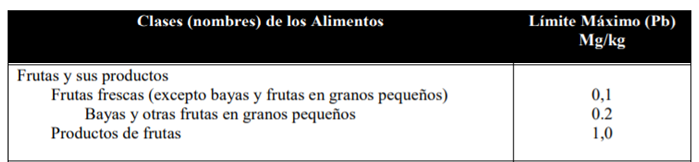
\includegraphics[keepaspectratio]{index_files/figure-html/figura7.png}}

}

\end{figure}%

\textbf{Químicos:} Esta norma establece los límites máximos en alimentos
de plomo, cadmio, mercurio, arsénico, estaño, níquel, cromo, nitrito,
nitrato, benzo (a) pireno, N- dimetilnitrosamina, Policlorobifenilos y
3-cloro-1, 2- propanodiol.

\paragraph{Normas de etiquetado.}\label{normas-de-etiquetado}

El etiquetado de alimentos preenvasados (todo alimento envuelto,
empaquetado o embalado previamente, listo para ofrecerlo al consumido)
se rige en China por la norma GB 7718 -- 2011 ``Norma General para
Etiquetado de Alimentos Preenvasados.

\begin{itemize}
\item
  Deberá ser de conformidad con los requisitos de las leyes estatales y
  reglamentos, así como con las normas de seguridad alimentaria.
\item
  Tendrá que ser claro, llamativo y duradero. Debe ser fácilmente
  legible e identificable por los consumidores al comprarlo.
\item
  Deberá ser verdadero, exacto, y no deberá presentar alimentos de
  manera falsa, exagerada, confundir a los consumidores ni con palabras
  o imágenes engañosas.
\item
  No deberá describirse ni presentarse con palabras, imágenes o símbolos
  que se refieran o se sugieran, directa o indirectamente, a cualquier
  otro producto.
\item
  Deberá utilizar los caracteres chinos estándares (salvo en la marca).
  Todas las lenguas extranjeras no pueden ser mayores que los caracteres
  chinos correspondientes (salvo la marca).
\end{itemize}

\paragraph{Normas de envases y
embalajes.}\label{normas-de-envases-y-embalajes}

En China, los envases y embalajes están regulados por la ley de
Seguridad Alimentaria publicada en el 2009. Los artículos N° 32 y N° 62
prohíben la importación, uso o compra de aditivos, materiales de envases
que no cumplan con los estándares chinos de seguridad alimentaria.

\paragraph{Normas ambientales.}\label{normas-ambientales}

Dentro de las Normas que actualmente están funcionando en China en el
ámbito ambiental (clima y biodiversidad) para frutas y verduras frescas
y fabricación de productos alimentarios (procesados) esta:

\textbf{IFOAM Basic Standard}/ \textbf{GB 2760 -- 2011}

\subsection{Canales de distribución}\label{canales-de-distribuciuxf3n}

\begin{figure}[H]

\caption{Canales de distribución}

{\centering \pandocbounded{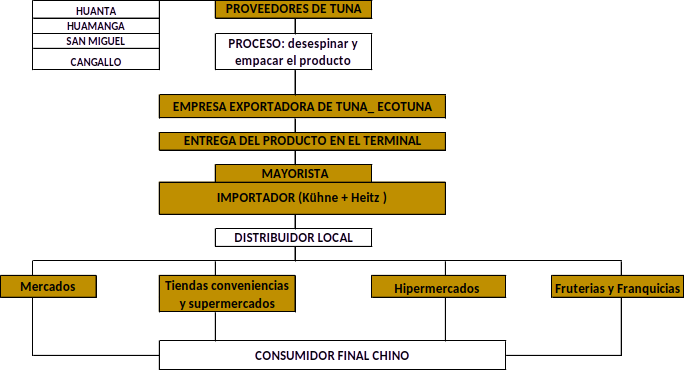
\includegraphics[keepaspectratio]{index_files/figure-html/figura8.png}}

}

\end{figure}%

El canal de distribución de la empresa exportadora ECO\emph{TUNA será
por medio del \_canal mayorista,} el producto ira del exportador a manos
del mayorista o distribuidor general, luego pasará por un minorista o
distribuidor local para llegar al consumidor final, de la siguiente
forma:

Exportador---------\textgreater{} Mayorista--------\textgreater{}
Minoristas---------\textgreater{} Usuario

\subsection{Medio de transporte}\label{medio-de-transporte}

El medio de transporte para la exportación de Tuna blanca y naranja se
realiza a través del Transporte aéreo, se llevará el producto vía aérea
porque es un transporte rápido, ideal para productos perecibles y con
alto grado de fragilidad como la tuna.

\subsection{Análisis de la demanda}\label{anuxe1lisis-de-la-demanda}

\subsubsection{Tendencia general del
consumidor}\label{tendencia-general-del-consumidor}

\begin{figure}[!htbp]

{\caption{{Segmentación demográfica}{\label{fig-myimportedimagesd}}}}

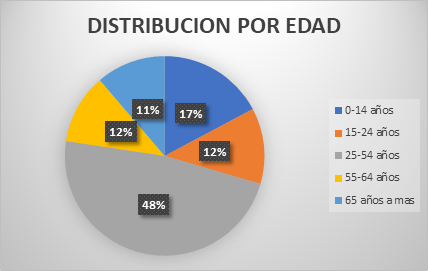
\includegraphics[width=5in,height=\textheight,keepaspectratio]{index_files/figure-html/figura9.png}

{\noindent \emph{Note.} Indexmundi, elaboración propia}

\end{figure}

Si bien es cierto que nuestro producto puede ser consumido por todos los
rangos de edades, nuestra población objetivo será la de 25-54 años ya
que conforman el mayor porcentaje de la población y a su ves
consideramos que dentro de estos rangos de edades se encuentran las
personas con más independencia económica o con familias para adquirir
nuestro producto.

\begin{figure}[!htbp]

{\caption{{Segmentación socioeconómica}{\label{fig-myimportedimagess}}}}

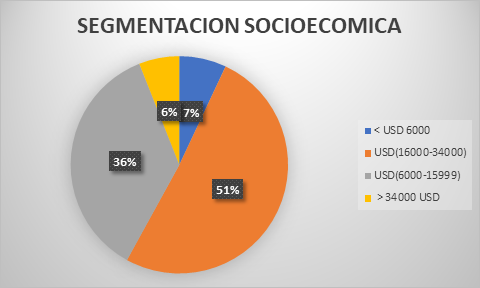
\includegraphics[width=5in,height=\textheight,keepaspectratio]{index_files/figure-html/figura10.png}

{\noindent \emph{Note.} Mckinsey quarterly, elaboracion propia}

\end{figure}

Nuestro producto ira dirigido a personas con ingresos de entre
16000-34000 USD pues conforman el mayor porcentaje de la población

\begin{figure}[!htbp]

{\caption{{Segmentación geográfica}{\label{fig-myimportedimagesg}}}}

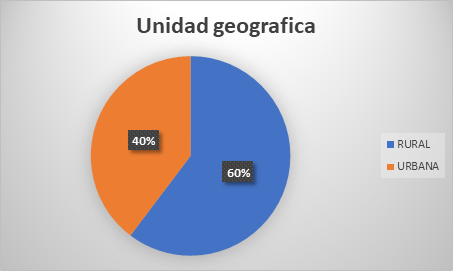
\includegraphics[width=5in,height=\textheight,keepaspectratio]{index_files/figure-html/figura11.png}

{\noindent \emph{Note.} Santader trade elaboracion propia}

\end{figure}

\begin{figure}[!htbp]

{\caption{{Consumo percapita anual de fruta por ciudad
(2017)}{\label{fig-myimportedimagecpadfpc}}}}

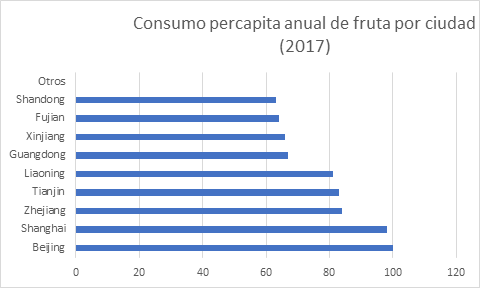
\includegraphics[width=5in,height=\textheight,keepaspectratio]{index_files/figure-html/figura12.png}

{\noindent \emph{Note.} National Bureau of Statistics of China
elaboración Propia}

\end{figure}

Nuestro mercado objetivo será la población urbana centrada en la ciudad
de Beijing ya que tiene el consumo per cápita anual más grande de fruta
en china.

\subsection{Características generales del
mercado}\label{caracteruxedsticas-generales-del-mercado}

FACTOR DEMOGRÁFICO: China cuenta con una población de 1.400.050.000 de
habitantes, ``siendo el país más poblado del mundo, tiene una densidad
de población media, de 146 habitantes por Km2'' (Datos,2018). La
conformación de la población no es diversa, Tan solo un 0,07\% de la
población de China son inmigrantes, según los últimos datos de
inmigración publicados por la ONU.

FACTOR ECONÓMICO: China es la segunda economía del mundo por volumen de
PIB (15255791.88 mill USD). Además es el segundo país con mayor volumen
de importaciones del ranking mundial, los compradores chinos están
interesados en importar fruta de todo el mundo fundamentalmente del
hemisferio sur, las que distribuye en el mercado mayorista, en tiendas
de frutas como (Gogo Fruits) comercializada través de una plataforma de
`e-commerce', asi también como la italiana RK Growers que busca
posicionarse en China con un amplio catálogo de productos, producidos en
Italia, pero también en países del hemisferio sur.

FACTOR ESTILO DE VIDA: Este es un factor clave pues a medida que mejoran
las condiciones de vida en China, el número de pacientes de alta presión
arterial, alto nivel de glucemia y alta grasa sanguínea se incrementa
cada día más, por lo que se espera que los ciudadanos cambien y
reajusten sus hábitos alimenticios, así como aumenten la variedad de
frutas que consumen. La Tuna podría satisfacer esta demanda ya que esta
posee un alto valor nutricional, es considerado un alimento funcional ya
que su consumo proporciona beneficios que fortalecen la salud , es alto
en fibra ,poder antioxidante y rica en vitamina C por lo que su consumo
evita el envejecimiento de los tejidos , ayuda a la prevención de la
obesidad diabetes y al control del colesterol.(Organización para las
Naciones Unidas para la Alimentación {[}FAO{]},2016),

FACTOR TECNOLÓGICO: Debido a que el día a día de la población China
transcurre de una forma muy rápida, éstos buscan opciones que se acoplen
a su velocidad, no dejando de lado la calidad de lo que desean adquirir.
Por tal razón, las ventas por internet y aplicaciones móviles se han
incrementado ya que esta forma de compra les garantiza el consumo
instantáneo (Promperú, 2015).

\subsection{Análisis del comportamiento del
consumidor}\label{anuxe1lisis-del-comportamiento-del-consumidor}

Los consumidores chinos están cada vez más concienciados hacia hábitos
de vida más saludables, por el aumento de enfermedades vinculadas a los
estilos de vida, actualmente se observa una preocupación entre la
población por incluir en sus dietas alimentos más saludables, entre los
que destacan los productos vegetales frescos y, en especial, las frutas.
La Tuna podría satisfacer esta demanda ya que ``la tuna posee un alto
valor en fibra ,poder antioxidante y es rica en vitamina C por lo que su
consumo evita el envejecimiento de los tejidos , ayuda a la prevención
de la obesidad diabetes y al control del colesterol.(Organización para
las Naciones Unidas para la Alimentación'' (FAO,2016).Por otro lado, es
preciso indicar que ``el consumidor Chino está dispuesto a probar
productos novedosos y de sabores regionales, ya que éstos les otorgan
una mayor variedad al momento de elegir un alimento pero sin embargo es
necesario que cuando una fruta es `desconocida' para el grueso de la
población, hay que facilitarle la tarea de comerla. Y si viene bien
presentada, mucho mejor'' (Redagricola,2018).Por otro lado de acuerdo a
Bain \& Company, cerca del 70\% de los compradores `online' escribe
`reviews' sobre los productos que ha comprado, mientras que el 90\% de
los compradores lee `reviews' antes de realizar una compra, El
consumidor chino es cada día más exigente y cada vez pide más calidad,
tiene predilección por frutas lustrosas, con colores vivos y uniformes.

Además, existe una demanda de fruta fresca fuertemente relacionado con
el mercado del regalo, ya que las frutas se usan como obsequio en las
principales fiestas del país, en bodas y celebraciones, para pacientes
en hospitales y en ocasiones especiales. Por este motivo, la mejor época
para la venta de fruta importada es la celebración del Año Nuevo Chino,
entre los meses de enero y febrero; y el Festival de Otoño entre
septiembre y octubre. Durante estas fiestas se comercializa un gran
volumen de fruta importada.

\section{Capítulo 4. Plan de
operación}\label{capuxedtulo-4.-plan-de-operaciuxf3n}

\subsection{Ficha de insumo producto}\label{ficha-de-insumo-producto}

\subsubsection{Insumos}\label{insumos}

Materia prima: Tuna que es alto en fibra, tiene antioxidante y rica en
vitamina C por lo que su consumo evita el envejecimiento de los tejidos,
ayuda a la prevención de la obesidad diabetes y control del colesterol.

\subsubsection{Personal}\label{personal}

\begin{itemize}
\tightlist
\item
  Mano de obra indirecta

  \begin{itemize}
  \tightlist
  \item
    1 gerente
  \item
    1 secretaria, recepcionista
  \end{itemize}
\item
  mano de obra directa

  \begin{itemize}
  \tightlist
  \item
    5 encargados del área de empaque
  \end{itemize}
\end{itemize}

En conclusión, para el normal funcionamiento de la empresa se requerirán
7 personas en su totalidad, para administración, operación, seguridad y
limpieza

\subsubsection{Costos de producción}\label{costos-de-producciuxf3n}

\begin{longtable}[]{@{}lc@{}}
\toprule\noalign{}
\textbf{Costo variable} & \textbf{Soles} \\
\midrule\noalign{}
\endhead
\bottomrule\noalign{}
\endlastfoot
Materia prima e insumos & 12672 \\
Mano de obra & 100 \\
\textbf{Total costo variable} & \textbf{12772} \\
Costo total & 12772.00 \\
Unidades & 1500 \\
Costo variable unitario & 8.51 \\
Costo total unitario & 8.515 \\
Margen de ganancia 80\% & 6.8117 \\
Precio & 15.33 \\
Precio exportador & 22989.6 \\
\end{longtable}

\subsection{Cadena de producción}\label{cadena-de-producciuxf3n}

Flujo del proceso productivo de la tuna

\begin{enumerate}
\def\labelenumi{\arabic{enumi}.}
\item
  Recepción de la tuna cosechada
\item
  Limpieza y cepillado
\item
  Inspección y selección
\item
  clasificación
\item
  Colocación del papel enserado
\item
  Colocación en cubetas
\item
  Colocación cajas
\item
  Carga al camión
\item
  Entrega en el aeropuerto
\end{enumerate}

\section{Capítulo 5. Gestión
exportadora}\label{capuxedtulo-5.-gestiuxf3n-exportadora}

\subsection{Análisis de Costos y precios de
exportación}\label{anuxe1lisis-de-costos-y-precios-de-exportaciuxf3n}

\begin{table}

{\caption{{Plan para la internacionalización del
nopal}{\label{tbl-mytablePPLIDN}}}}

\begin{longtable}[]{@{}
  >{\raggedright\arraybackslash}p{(\linewidth - 6\tabcolsep) * \real{0.2297}}
  >{\centering\arraybackslash}p{(\linewidth - 6\tabcolsep) * \real{0.2297}}
  >{\raggedright\arraybackslash}p{(\linewidth - 6\tabcolsep) * \real{0.3108}}
  >{\raggedright\arraybackslash}p{(\linewidth - 6\tabcolsep) * \real{0.2297}}@{}}
\toprule\noalign{}
\begin{minipage}[b]{\linewidth}\raggedright
\textbf{Detalles}
\end{minipage} & \begin{minipage}[b]{\linewidth}\centering
\textbf{I}
\end{minipage} & \begin{minipage}[b]{\linewidth}\raggedright
\textbf{Producto: nombre técnico o comercial}
\end{minipage} & \begin{minipage}[b]{\linewidth}\raggedright
\textbf{TUNA O NOPAL}
\end{minipage} \\
\midrule\noalign{}
\endhead
\bottomrule\noalign{}
\endlastfoot
Información básica del producto & II & Posición arancelaria del país
exportador & 810909000 \\
& & Posición arancelaria del país importador & 81340 \\
& III & Unidad comercial de venta & KILO \\
& IV & Valor por unidad comercial & \$0.63 \\
& V & Empaque & CAJAS \\
& & Dimensiones de cajas & 0.60\emph{0.38}0.16 \\
Información básica del embarque & VI & Origen/país punto de carga &
Ayacucho/Callao \\
& VII & Destino /país punto de desembarque & Beijing/China \\
& VIII & Peso total & 55000 \\
& IX & Unidad de carga & CAJAS \\
& X & Unitarización & UNITARIZADO 1 CONT.X40''RF \\
& XI & Cantidad total de cajas & 2500 \\
& XII & Unidades comerciales & 52500 \\
Otra información de importancia & XIII & Valor total mercancía &
\$33,011.36 \\
& XIV & Forma de pago y tiempo & Anticipado giro directo \\
& XV & Tipo de cambio actualizado & 3.96 \\
\end{longtable}

\end{table}

\begin{table}

{\caption{{FCA}{\label{tbl-mytableFCA}}}}

\begin{longtable}[]{@{}lc@{}}
\toprule\noalign{}
& \textbf{FCA} \\
\midrule\noalign{}
\endhead
\bottomrule\noalign{}
\endlastfoot
Total exportador & 167704 \\
Total importador & 1401434 \\
Costo unitario exportador & 67.082 \\
Precio unitario al importador & 134.163 \\
Precio total al importador (Valor Factura) & 335,408 \\
\end{longtable}

\end{table}

\subsection{Modalidades de pago}\label{modalidades-de-pago}

\subsubsection{Forma de pago}\label{forma-de-pago}

La empresa ECOTUNA tendrá la modalidad de pago por adelantado del 50\% y
como institución intermediaria será INTERBANK, en vista de que esta
forma de pago es la más segura teniendo en cuenta aspectos de riesgo.

\begin{longtable}[]{@{}ll@{}}
\toprule\noalign{}
\textbf{Medio/forma de pago} & \textbf{Riesgo exportador} \\
\midrule\noalign{}
\endhead
\bottomrule\noalign{}
\endlastfoot
Pago por adelantado & Ninguno \\
Carta de crédito & Discrepancias documentarias \\
Cobranza documentaria & No pago /no aceptación \\
Cobranza simple & Solvencia del importador \\
Cuenta & Máximo \\
\end{longtable}

\subsubsection{Entrega de mercancía}\label{entrega-de-mercancuxeda}

Según el ministerio de desarrollo agrario y riego con el incoterm FCA,
Free Carrier (Libre Transportista) el exportador entrega la mercancía en
el lugar acordado por ello la empresa se compromete a cumplir sus
obligaciones como exportador.

\subsubsection{Cobro}\label{cobro}

La modalidad de cobro de la empresa ECOTUNA que corresponde al 50\% se
realizara de forma efectiva después de la transferencia de la mercancía
a nuestro cliente y en el mismo lugar

\subsection{Riesgos}\label{riesgos}

El Seguro de Crédito a la Exportación es un mecanismo de coberturas que
protege a los exportadores contra los Riesgos Ordinarios y
Extraordinarios del Comercio Internacional permitiendo a los mismos
resarcirse de los daños ocasionados por determinados acontecimientos que
pudieren impedir el cobro o recuperación de los créditos acordados a sus
compradores en el exterior. En este sentido la empresa Ecotuna S.C.R.L
contrata a COFACE for trade una compañía Aseguradora para obtener un
seguro de crédito a la exportación, el cual cubrirá los riesgos de
rescisión o resolución del contrato y el riesgo de impago.

\begin{enumerate}
\def\labelenumi{\arabic{enumi}.}
\setcounter{enumi}{10}
\tightlist
\item
  Información adicional:
\end{enumerate}

Datos de importadores:

\begin{longtable}[]{@{}
  >{\raggedright\arraybackslash}p{(\linewidth - 2\tabcolsep) * \real{0.3889}}
  >{\raggedright\arraybackslash}p{(\linewidth - 2\tabcolsep) * \real{0.6111}}@{}}
\toprule\noalign{}
\begin{minipage}[b]{\linewidth}\raggedright
\textbf{Empresa}
\end{minipage} & \begin{minipage}[b]{\linewidth}\raggedright
\textbf{SOUSA RIBEIRO AGRAO TRADE EXPORT}
\end{minipage} \\
\midrule\noalign{}
\endhead
\bottomrule\noalign{}
\endlastfoot
Representante & CORREA MIRANDA SOUSA ALFREDO EDUARDO \\
Industria & Comercio de frutas y plantas medicinales \\
Escala comercial & Empresas líderes de alto potencial \\
Dirección & Av. Stanislas Pryl, 11145435-000 Ituberá / BA Brasil \\
Productos & Guaraná, cacao, pimentón brasileño, pasiflora, secula de
topioca, pupunha, nuez de Brasil y aceites esenciales. \\
Código hs & 020714SUDU817722700 \\
Cantidad de empleados & 1001 \\
Teléfono fax & +55 73 3256-2705 \\
Sitio web &
\href{mailto:atendimento@sousaribeiro.com.br}{Atendimento@sousaribeiro.com.br} \\
Ranking de mercados top & \\
& Estados unidos \\
& Argentina \\
& Reino unido \\
Volumen de importación & USD\$125 millones \\
\end{longtable}

\begin{longtable}[]{@{}
  >{\raggedright\arraybackslash}p{(\linewidth - 2\tabcolsep) * \real{0.3889}}
  >{\raggedright\arraybackslash}p{(\linewidth - 2\tabcolsep) * \real{0.6111}}@{}}
\toprule\noalign{}
\begin{minipage}[b]{\linewidth}\raggedright
\textbf{Empresa}
\end{minipage} & \begin{minipage}[b]{\linewidth}\raggedright
\textbf{Maripa Importacao e Exportacao}
\end{minipage} \\
\midrule\noalign{}
\endhead
\bottomrule\noalign{}
\endlastfoot
Representante & Tatiana amaral torrinha balducci 22-sócio \\
Industria & Concervas de frutas y frutas \\
Escala comercial & Líderes de alto potencial \\
Dirección & Extensión Unifap Y / N KM 02 Highway jk Barrio: Jardim Marco
Zero Municipio: Macapa Estado: AP \\
Productos & Cereza, mango, manzana, quiwi, pomelos \\
Código hs & 24.283.272/0001-04 \\
Cantidad de empleados & 1123 \\
Teléfono fax & (96) 9181-3939 / (96) 9135-0324 \\
Sitio web &
\url{Https://cnpjs.rocks/cnpj/24283272000104/maripa-importacao-e-exportacao-ltda.html} \\
Ranking de mercados top & \\
& Argentina \\
& Perú \\
& México \\
Volumen de importación & US\$ 138 millones \\
\end{longtable}

\subsection{Ferias}\label{ferias}

\subsubsection{Fruit \& Tech}\label{fruit-tech}

Fruit \& Tech~brinda al mercado productor de~frutas, verduras y
derivados, tecnología y logística~todas las condiciones para
la~generación de negocios, ampliación de contactos comerciales, apertura
al mercado externo y aumento de ventas.

Con amplia presencia de compradores internacionales, el evento destaca
las rondas de negocios, seminarios, lanzamiento de productos, difusión
de técnicas y nuevas tecnologías, entre otras atracciones.

\subsubsection{Frutal}\label{frutal}

\textbf{Frutal}~se celebra anualmente en diciembre y atrae a visitantes
de todo Brasil~y de otros países, que asisten al evento para~conocer
las~últimas novedades del sector de las frutas, las flores y la
agroindustria. El evento reúne~productores, importadores y proveedores
de servicios para el sector, además de técnicos, entidades públicas,
maquinaria y demás profesionales de la cadena de suministro.

\subsubsection{Expo Fruit}\label{expo-fruit}

El~Exprofuit~es una de las ferias más importantes en el sector de las
frutas que está sucediendo en Brasil. Pretende reunir a los productores
de frutas de regadío y de otros eslabones de la cadena, como
importadores, exportadores, distribuidores, proveedores, y las
delegaciones de países como Francia, Italia, Alemania, España, Países
Bajos, República Checa, Bélgica, Noruega, EE.UU., Rusia, entre otros
para realizar negocios.

\section{Capítulo 6}\label{capuxedtulo-6}

\subsection{Análisis comparativos de precios de
Brasil}\label{anuxe1lisis-comparativos-de-precios-de-brasil}

\begin{table}

{\caption{{Valor de exportación con incoterm
CPT}{\label{tbl-mytableVDECI}}}}

\begin{longtable}[]{@{}
  >{\raggedright\arraybackslash}p{(\linewidth - 4\tabcolsep) * \real{0.4722}}
  >{\raggedright\arraybackslash}p{(\linewidth - 4\tabcolsep) * \real{0.2778}}
  >{\raggedright\arraybackslash}p{(\linewidth - 4\tabcolsep) * \real{0.2500}}@{}}
\toprule\noalign{}
\begin{minipage}[b]{\linewidth}\raggedright
\textbf{Costos}
\end{minipage} & \begin{minipage}[b]{\linewidth}\raggedright
\textbf{Documentación}
\end{minipage} & \begin{minipage}[b]{\linewidth}\raggedright
\textbf{CPT}
\end{minipage} \\
\midrule\noalign{}
\endhead
\bottomrule\noalign{}
\endlastfoot
Costos de producción & \textsc{\textbf{FACTURA COMERCIAL}} & 22,990 \\
Flete terrestre 40's (17 unidades) & \textsc{\textbf{CARTA PORTE}} &
1,000 \\
Derechos de trámite aduanero & \textsc{\textbf{DTA-PEDIMIENTO DE X}} &
1,839 \\
Honorarios de AA Exp & \textsc{\textbf{CUENTA DE GASTOS AA}} & 395 \\
Maniobras de carga & \textsc{\textbf{TICKET DE MANIOBRAS}} & 700 \\
Total exportador & & 26,924 \\
Costo unitario exportador & & 17.9491787 \\
Precio total al importador precio total. & & 35.8983573 \\
& & \\
\end{longtable}

\end{table}

\begin{table}

{\caption{{Valor de exportación CIF -- costo de la tuna en el puerto de
Sao Paulo}{\label{tbl-mytable}}}}

\begin{longtable}[]{@{}
  >{\raggedright\arraybackslash}p{(\linewidth - 6\tabcolsep) * \real{0.2222}}
  >{\raggedright\arraybackslash}p{(\linewidth - 6\tabcolsep) * \real{0.3333}}
  >{\raggedright\arraybackslash}p{(\linewidth - 6\tabcolsep) * \real{0.2222}}
  >{\raggedright\arraybackslash}p{(\linewidth - 6\tabcolsep) * \real{0.2222}}@{}}
\toprule\noalign{}
\begin{minipage}[b]{\linewidth}\raggedright
\textbf{DESCRIPCIÓN}
\end{minipage} & \begin{minipage}[b]{\linewidth}\raggedright
\textbf{PRECIO UNITARIO CPT BRASIL US\$}
\end{minipage} & \begin{minipage}[b]{\linewidth}\raggedright
\textbf{CANTIDADES UNIDADES}
\end{minipage} & \begin{minipage}[b]{\linewidth}\raggedright
\textbf{TOTAL CPT}
\end{minipage} \\
\midrule\noalign{}
\endhead
\bottomrule\noalign{}
\endlastfoot
MODELO A & 17.94917867 & 1500 & 26923.77 \\
& & TOTAL CPT Brasil & 26923.77 \\
& & FLETE AÉREO & 1154.74 \\
& & SEGURO & 592.5 \\
& & TOTAL CIF & \$ 28,671.01 \\
\end{longtable}

\end{table}

\_

\begin{longtable}[]{@{}ll@{}}
\caption{Costos de importación en Brasil\_}\tabularnewline
\toprule\noalign{}
\textbf{CTM(US\$)} & \textbf{\$ 39,959.09} \\
\midrule\noalign{}
\endfirsthead
\toprule\noalign{}
\textbf{CTM(US\$)} & \textbf{\$ 39,959.09} \\
\midrule\noalign{}
\endhead
\bottomrule\noalign{}
\endlastfoot
FACTOR DE CALCULO & 1.48 \\
\end{longtable}

El costo de la tuna se incremento en 0.48 céntimos de soles

\begin{longtable}[]{@{}
  >{\centering\arraybackslash}p{(\linewidth - 10\tabcolsep) * \real{0.1667}}
  >{\centering\arraybackslash}p{(\linewidth - 10\tabcolsep) * \real{0.1667}}
  >{\centering\arraybackslash}p{(\linewidth - 10\tabcolsep) * \real{0.1667}}
  >{\centering\arraybackslash}p{(\linewidth - 10\tabcolsep) * \real{0.1667}}
  >{\centering\arraybackslash}p{(\linewidth - 10\tabcolsep) * \real{0.1667}}
  >{\centering\arraybackslash}p{(\linewidth - 10\tabcolsep) * \real{0.1667}}@{}}
\caption{Precio en dólares en Brasil}\tabularnewline
\toprule\noalign{}
\begin{minipage}[b]{\linewidth}\centering
\textbf{Factor de distribución}
\end{minipage} & \begin{minipage}[b]{\linewidth}\centering
\textbf{Costo unitario de importación}
\end{minipage} & \begin{minipage}[b]{\linewidth}\centering
\textbf{P margen de ganancia 30\%}
\end{minipage} & \begin{minipage}[b]{\linewidth}\centering
\textbf{Iva 19\%}
\end{minipage} & \begin{minipage}[b]{\linewidth}\centering
\textbf{Precio soles}
\end{minipage} & \begin{minipage}[b]{\linewidth}\centering
\textbf{Precio-dólares}
\end{minipage} \\
\midrule\noalign{}
\endfirsthead
\toprule\noalign{}
\begin{minipage}[b]{\linewidth}\centering
\textbf{Factor de distribución}
\end{minipage} & \begin{minipage}[b]{\linewidth}\centering
\textbf{Costo unitario de importación}
\end{minipage} & \begin{minipage}[b]{\linewidth}\centering
\textbf{P margen de ganancia 30\%}
\end{minipage} & \begin{minipage}[b]{\linewidth}\centering
\textbf{Iva 19\%}
\end{minipage} & \begin{minipage}[b]{\linewidth}\centering
\textbf{Precio soles}
\end{minipage} & \begin{minipage}[b]{\linewidth}\centering
\textbf{Precio-dólares}
\end{minipage} \\
\midrule\noalign{}
\endhead
\bottomrule\noalign{}
\endlastfoot
1.48 & 26.64 & 34.63 & 6.58 & 41.21 & 10.43 \\
& & & Precio promedio & 41.21 & \$ 10.43 \\
Precio internacional & 11.7721519 & & & & \\
\end{longtable}

Si sería rentable pues nuestro precio promedio es 10.43 dólares el cual
es menor al precio del mercado internacional de 11.72 dólares , por lo
que somos competitivos en el exterior con un margen de ganancia de
100\%.

\section{Publicaciones Similares}\label{publicaciones-similares}

Si te interesó este artículo, te recomendamos que explores otros blogs y
recursos relacionados que pueden ampliar tus conocimientos. Aquí te dejo
algunas sugerencias:

\begin{enumerate}
\def\labelenumi{\arabic{enumi}.}
\tightlist
\item
  \href{https://achalmaedison.netlify.app/blog/posts/2015-05-14-el-aborto/index.pdf}{\faIcon{file-pdf}}
  \href{https://achalmaedison.netlify.app/blog/posts/2015-05-14-el-aborto}{El
  Aborto}
\item
  \href{https://achalmaedison.netlify.app/blog/posts/2017-04-23-sitios-web-asombrosos/index.pdf}{\faIcon{file-pdf}}
  \href{https://achalmaedison.netlify.app/blog/posts/2017-04-23-sitios-web-asombrosos}{Sitios
  Web Asombrosos}
\item
  \href{https://achalmaedison.netlify.app/blog/posts/2017-05-23-el-mercantilismo/index.pdf}{\faIcon{file-pdf}}
  \href{https://achalmaedison.netlify.app/blog/posts/2017-05-23-el-mercantilismo}{El
  Mercantilismo}
\item
  \href{https://achalmaedison.netlify.app/blog/posts/2020-05-23-comandos-de-google-assistant/index.pdf}{\faIcon{file-pdf}}
  \href{https://achalmaedison.netlify.app/blog/posts/2020-05-23-comandos-de-google-assistant}{Comandos
  De Google Assistant}
\item
  \href{https://achalmaedison.netlify.app/blog/posts/2020-09-15-plan-de-negocio-exportacion-de-trucha-arcoires/index.pdf}{\faIcon{file-pdf}}
  \href{https://achalmaedison.netlify.app/blog/posts/2020-09-15-plan-de-negocio-exportacion-de-trucha-arcoires}{Plan
  De Negocio Exportacion De Trucha Arcoires}
\item
  \href{https://achalmaedison.netlify.app/blog/posts/2021-07-13-plan-de-negocio-exportacion-de-tuna/index.pdf}{\faIcon{file-pdf}}
  \href{https://achalmaedison.netlify.app/blog/posts/2021-07-13-plan-de-negocio-exportacion-de-tuna}{Plan
  De Negocio Exportacion De Tuna}
\item
  \href{https://achalmaedison.netlify.app/blog/posts/2021-07-14-comandos-de-blogdown/index.pdf}{\faIcon{file-pdf}}
  \href{https://achalmaedison.netlify.app/blog/posts/2021-07-14-comandos-de-blogdown}{Comandos
  De Blogdown}
\item
  \href{https://achalmaedison.netlify.app/blog/posts/2021-10-01-gestion-publica-y-administracion-publica/index.pdf}{\faIcon{file-pdf}}
  \href{https://achalmaedison.netlify.app/blog/posts/2021-10-01-gestion-publica-y-administracion-publica}{Gestion
  Publica Y Administracion Publica}
\item
  \href{https://achalmaedison.netlify.app/blog/posts/2021-10-01-reformas-y-modernizacion-de-la-gestion-publica/index.pdf}{\faIcon{file-pdf}}
  \href{https://achalmaedison.netlify.app/blog/posts/2021-10-01-reformas-y-modernizacion-de-la-gestion-publica}{Reformas
  Y Modernizacion De La Gestion Publica}
\item
  \href{https://achalmaedison.netlify.app/blog/posts/2022-01-23-cadena\%20de\%20suministros/index.pdf}{\faIcon{file-pdf}}
  \href{https://achalmaedison.netlify.app/blog/posts/2022-01-23-cadena\%20de\%20suministros}{Cadena
  De Suministros}
\item
  \href{https://achalmaedison.netlify.app/blog/posts/2022-04-22-economia-agraria/index.pdf}{\faIcon{file-pdf}}
  \href{https://achalmaedison.netlify.app/blog/posts/2022-04-22-economia-agraria}{Economia
  Agraria}
\item
  \href{https://achalmaedison.netlify.app/blog/posts/2022-06-02-impacto-del-cambio-climatico/index.pdf}{\faIcon{file-pdf}}
  \href{https://achalmaedison.netlify.app/blog/posts/2022-06-02-impacto-del-cambio-climatico}{Impacto
  Del Cambio Climatico}
\item
  \href{https://achalmaedison.netlify.app/blog/posts/2023-05-11-cualidades-de-los-servidores-publicos/index.pdf}{\faIcon{file-pdf}}
  \href{https://achalmaedison.netlify.app/blog/posts/2023-05-11-cualidades-de-los-servidores-publicos}{Cualidades
  De Los Servidores Publicos}
\item
  \href{https://achalmaedison.netlify.app/blog/posts/2023-05-12-la-economia-peruana-entre-1970-1990/index.pdf}{\faIcon{file-pdf}}
  \href{https://achalmaedison.netlify.app/blog/posts/2023-05-12-la-economia-peruana-entre-1970-1990}{La
  Economia Peruana Entre 1970 1990}
\item
  \href{https://achalmaedison.netlify.app/blog/posts/2023-05-16-economia-regional/index.pdf}{\faIcon{file-pdf}}
  \href{https://achalmaedison.netlify.app/blog/posts/2023-05-16-economia-regional}{Economia
  Regional}
\end{enumerate}

Esperamos que encuentres estas publicaciones igualmente interesantes y
útiles. ¡Disfruta de la lectura!






\end{document}
